\documentclass[11pt,a4paper]{article}

% ── Packages ──────────────────────────────────────────────────────
\usepackage[utf8]{inputenc}
\usepackage[T1]{fontenc}
\usepackage{amsmath,amssymb,amsfonts}
\usepackage{graphicx}
\usepackage{booktabs}
\usepackage{hyperref}
\usepackage{xcolor}
\usepackage{algorithm}
\usepackage{algorithmic}
\usepackage{listings}
\usepackage{geometry}
\usepackage{caption}
\usepackage{subcaption}
\usepackage{enumitem}
\usepackage{multirow}
\usepackage{tikz}
\usetikzlibrary{arrows.meta,positioning,shapes.geometric,fit,calc}
\usepackage{natbib}

\geometry{margin=2.5cm}

\lstset{
  basicstyle=\ttfamily\small,
  keywordstyle=\color{blue}\bfseries,
  commentstyle=\color{green!50!black},
  stringstyle=\color{red!70!black},
  breaklines=true,
  frame=single,
  numbers=left,
  numberstyle=\tiny\color{gray},
  xleftmargin=2em,
  framexleftmargin=1.5em,
}

% ── Title ─────────────────────────────────────────────────────────

\title{MI-Workbench: An Autonomous Multi-Agent Platform for\\Rigorous Mechanistic Interpretability Research}

\author{
  Ihor Kendiukhov \\
  \texttt{biodyn-research}
}

\date{February 2026}

\begin{document}
\maketitle

% ── Abstract ──────────────────────────────────────────────────────

\begin{abstract}
Mechanistic interpretability (MI) of biological foundation models---such as single-cell transformers trained on gene expression data---requires iterative cycles of hypothesis formation, experimental execution, statistical evaluation, and adversarial critique.
These cycles are labor-intensive, error-prone, and difficult to reproduce.
We present \textbf{MI-Workbench}, an open-source platform that orchestrates autonomous multi-agent research loops for MI investigations.
The system employs a graph-based domain-specific language (DSL) to define configurable workflows comprising executor, reviewer, adversarial reviewer, biological plausibility checker, and knowledge extractor agents.
Each agent is backed by a large language model (LLM) accessed through a provider-agnostic adapter layer supporting Claude Code, OpenAI Codex, and Google Gemini.
Key innovations include: (i)~a consensus reviewer mechanism that runs multiple critic agents in parallel, deduplicates findings via Jaccard similarity, and escalates severity when reviewers agree; (ii)~an output cleaning pipeline that strips LLM thinking traces from research artifacts; (iii)~structured feedback injection with artifact-level and section-level references that enables targeted revision rather than full rewriting; and (iv)~automated convergence detection, follow-up proposal generation, and reproducibility packaging.
We validate MI-Workbench on a case study investigating whether attention heads in the Geneformer single-cell foundation model encode causal gene regulatory relationships.
Across 11 end-to-end runs using the Gemini adapter, the platform produced scientifically rigorous protocols, identified key confounders (co-expression bias, rank-value encoding artifacts, attention symmetry), and iteratively refined analyses through structured feedback---all without human intervention.
The system comprises over 10,000 lines of Python, 360 passing tests, and supports real-time monitoring via WebSocket streaming.
\end{abstract}

% ── 1. Introduction ───────────────────────────────────────────────

\section{Introduction}
\label{sec:introduction}

The rapid development of biological foundation models---including scGPT~\citep{cui2024scgpt}, Geneformer~\citep{theodoris2023transfer}, and scBERT~\citep{yang2022scbert}---has raised fundamental questions about what these models learn and how their internal representations relate to known biology.
\emph{Mechanistic interpretability} (MI), the discipline of reverse-engineering the computational mechanisms within neural networks~\citep{olah2020zoom,elhage2022toy,conmy2023towards}, offers a principled framework for answering these questions.
However, applying MI to biological models presents unique challenges:

\begin{enumerate}[leftmargin=*]
  \item \textbf{Confounding structures.} Gene co-expression, regulatory network degree distributions, and expression magnitude biases create complex confound structures that require carefully controlled null models~\citep{pratapa2020benchmarking}.
  \item \textbf{Statistical rigor.} Claims about learned regulatory mechanisms require multiple testing correction, effect size reporting, confidence intervals, and proper null model comparison---standards often missing from initial analyses.
  \item \textbf{Iterative refinement.} MI investigations are inherently cyclical: an initial analysis reveals confounders, which motivate new controls, which reveal subtler effects, and so on.
  \item \textbf{Reproducibility.} Complex computational pipelines with many degrees of freedom are difficult to reproduce without meticulous documentation of parameters, data versions, and analytical choices.
\end{enumerate}

While individual LLMs have demonstrated impressive capability for scientific reasoning~\citep{romera2024mathematical,boiko2023autonomous}, single-agent approaches lack the adversarial pressure and structured quality control necessary for rigorous research.
A human researcher typically cycles between the roles of \emph{executor} (performing analysis), \emph{reviewer} (critiquing methodology), and \emph{devil's advocate} (searching for confounders and alternative explanations).

We introduce \textbf{MI-Workbench}, a platform that automates this multi-role research process.
Our key contributions are:

\begin{itemize}[leftmargin=*]
  \item A \textbf{graph-based workflow DSL} that enables researchers to define arbitrary multi-agent research loops with conditional execution, parallel branching, and configurable stop conditions.
  \item A \textbf{consensus reviewer mechanism} that runs independent critic agents in parallel and merges their findings through deduplication, severity escalation, and ranked output.
  \item A \textbf{structured feedback loop} that maps reviewer critiques to specific artifacts and sections, enabling targeted revision rather than wholesale rewriting.
  \item A \textbf{provider-agnostic adapter architecture} that abstracts over Claude Code, OpenAI Codex, and Google Gemini CLI backends through a common interface.
  \item An integrated \textbf{knowledge extraction} pipeline that mines research claims from artifacts, estimates uncertainty, and generates falsification tests.
  \item End-to-end \textbf{reproducibility packaging} that bundles artifacts, prompts, environment metadata, and analysis provenance into portable archives.
\end{itemize}

% ── 2. Related Work ───────────────────────────────────────────────

\section{Related Work}
\label{sec:related}

\paragraph{Autonomous scientific agents.}
The vision of AI-driven scientific discovery has been explored through systems like ChemCrow~\citep{bran2024chemcrow}, which chains LLM reasoning with chemistry tools, and Coscientist~\citep{boiko2023autonomous}, which demonstrated autonomous experimental design in chemistry.
SciAgents~\citep{ghafarollahi2024sciagents} explored multi-agent scientific reasoning using graph-based ontologies.
These systems focus primarily on wet-lab experimental design; MI-Workbench targets the distinct challenge of computational interpretability with its emphasis on statistical rigor and confound control.

\paragraph{Multi-agent LLM frameworks.}
Multi-agent debate and collaboration have been studied in frameworks such as CAMEL~\citep{li2023camel}, AutoGen~\citep{wu2023autogen}, and ChatDev~\citep{qian2024chatdev}.
MetaGPT~\citep{hong2023metagpt} introduced structured output schemas for software engineering agents.
CrewAI and LangGraph provide general-purpose agent orchestration.
MI-Workbench differs from these frameworks in its domain specialization: the agent roles, prompt templates, artifact types, and quality criteria are specifically designed for mechanistic interpretability research in computational biology.

\paragraph{Mechanistic interpretability.}
The MI field has produced foundational work on circuits~\citep{olah2020zoom}, induction heads~\citep{olsson2022context}, activation patching~\citep{meng2022locating}, and superposition~\citep{elhage2022toy}.
Recent work has applied MI concepts to biological transformers: Geneformer~\citep{theodoris2023transfer} and scGPT~\citep{cui2024scgpt} have been probed for gene regulatory network (GRN) inference capabilities.
However, these analyses are typically manual, one-shot investigations.
MI-Workbench provides the infrastructure to systematize and scale such investigations.

\paragraph{Scientific workflow systems.}
Systems like Galaxy~\citep{afgan2018galaxy}, Nextflow~\citep{ditommaso2017nextflow}, and Snakemake~\citep{molder2021sustainable} manage computational biology pipelines.
These tools orchestrate deterministic code execution; MI-Workbench orchestrates \emph{reasoning} via LLM agents, where outputs are non-deterministic and require quality assessment.

% ── 3. System Architecture ───────────────────────────────────────

\section{System Architecture}
\label{sec:architecture}

MI-Workbench follows a layered architecture (Figure~\ref{fig:architecture}) comprising: (i)~a \textbf{REST API} layer built on FastAPI with WebSocket support for real-time monitoring; (ii)~an \textbf{orchestration engine} that drives the multi-agent loop; (iii)~a \textbf{provider-agnostic adapter layer} that interfaces with LLM backends; and (iv)~\textbf{persistence and artifact management} via SQLite and a structured file system.

\begin{figure}[t]
\centering
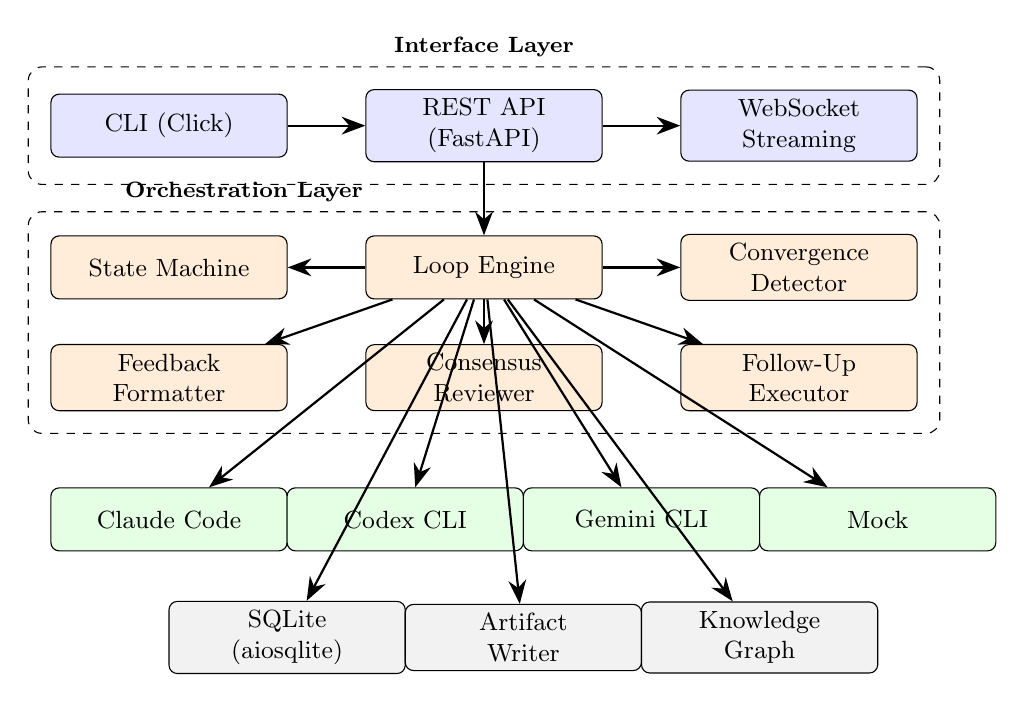
\begin{tikzpicture}[
  box/.style={rectangle, draw, rounded corners=3pt, minimum width=3cm, minimum height=0.8cm, align=center, font=\small},
  bigbox/.style={rectangle, draw, dashed, rounded corners=5pt, inner sep=8pt, align=center},
  arrow/.style={-{Stealth[length=3mm]}, thick},
  every node/.style={font=\small}
]

% CLI / API layer
\node[box, fill=blue!10] (cli) at (0, 6) {CLI (Click)};
\node[box, fill=blue!10] (api) at (4, 6) {REST API\\(FastAPI)};
\node[box, fill=blue!10] (ws) at (8, 6) {WebSocket\\Streaming};

% Engine layer
\node[box, fill=orange!15] (engine) at (4, 4.2) {Loop Engine};
\node[box, fill=orange!15] (sm) at (0, 4.2) {State Machine};
\node[box, fill=orange!15] (conv) at (8, 4.2) {Convergence\\Detector};
\node[box, fill=orange!15] (fb) at (0, 2.8) {Feedback\\Formatter};
\node[box, fill=orange!15] (cons) at (4, 2.8) {Consensus\\Reviewer};
\node[box, fill=orange!15] (fu) at (8, 2.8) {Follow-Up\\Executor};

% Adapter layer
\node[box, fill=green!10] (claude) at (0, 1.0) {Claude Code};
\node[box, fill=green!10] (codex) at (3, 1.0) {Codex CLI};
\node[box, fill=green!10] (gemini) at (6, 1.0) {Gemini CLI};
\node[box, fill=green!10] (mock) at (9, 1.0) {Mock};

% Persistence layer
\node[box, fill=gray!10] (db) at (1.5, -0.5) {SQLite\\(aiosqlite)};
\node[box, fill=gray!10] (artifacts) at (4.5, -0.5) {Artifact\\Writer};
\node[box, fill=gray!10] (knowledge) at (7.5, -0.5) {Knowledge\\Graph};

% Grouping boxes
\node[bigbox, fit=(cli)(api)(ws), label={[font=\footnotesize\bfseries]above:Interface Layer}] {};
\node[bigbox, fit=(engine)(sm)(conv)(fb)(cons)(fu), label={[font=\footnotesize\bfseries]above left:Orchestration Layer}] {};

% Arrows
\draw[arrow] (cli) -- (api);
\draw[arrow] (api) -- (engine);
\draw[arrow] (api) -- (ws);
\draw[arrow] (engine) -- (sm);
\draw[arrow] (engine) -- (conv);
\draw[arrow] (engine) -- (fb);
\draw[arrow] (engine) -- (cons);
\draw[arrow] (engine) -- (fu);
\draw[arrow] (engine) -- (claude);
\draw[arrow] (engine) -- (codex);
\draw[arrow] (engine) -- (gemini);
\draw[arrow] (engine) -- (mock);
\draw[arrow] (engine) -- (db);
\draw[arrow] (engine) -- (artifacts);
\draw[arrow] (engine) -- (knowledge);

\end{tikzpicture}
\caption{MI-Workbench architecture. The system comprises four layers: an interface layer (CLI, REST API, WebSocket), an orchestration layer (loop engine with state machine, convergence detection, feedback formatting, consensus review, and follow-up generation), a provider-agnostic adapter layer, and a persistence layer.}
\label{fig:architecture}
\end{figure}

\subsection{Workspace Model}
A \emph{workspace} represents an isolated research context with its own configuration, provider settings, budget limits, and git integration mode.
Each workspace contains one or more \emph{runs}, where each run executes a loop definition against a specific research task.
Runs produce versioned \emph{artifacts} organized by iteration: mechanistic analysis (\texttt{MECH.md}), evaluation reports (\texttt{EVAL.md}), experimental protocols (\texttt{XP.md}), methodology documentation (\texttt{METHOD.md}), and knowledge summaries (\texttt{KNOWLEDGE.md}).

\subsection{Data Model}
The system uses Pydantic~\citep{pydantic} for all data validation and serialization.
Key models include \texttt{RunState} (tracking run lifecycle, iterations, token usage, and cost), \texttt{IterationResult} (individual step outcomes with artifacts and feedback), \texttt{ReviewResult} (structured critique with severity levels and artifact references), and \texttt{LoopDefinition} (graph-based workflow specification).

% ── 4. Workflow DSL ───────────────────────────────────────────────

\section{Graph-Based Workflow DSL}
\label{sec:dsl}

MI-Workbench defines research workflows as directed graphs where nodes represent agent roles and edges encode execution flow with conditions.

\subsection{Loop Definition}
A loop definition consists of \emph{nodes} and \emph{edges} specified in YAML:

\begin{lstlisting}[language=Python,caption={Excerpt from the \texttt{executor\_reviewer} loop definition.}]
nodes:
  - id: executor
    role: executor
    prompt_ref: "executor/mi_executor"
  - id: reviewer
    role: reviewer
    prompt_ref: "reviewer/mi_reviewer"
  - id: adversarial
    role: adversarial_reviewer
    prompt_ref: "adversarial_reviewer/adversarial_reviewer"
edges:
  - source: executor
    target: reviewer
    condition: "always"
  - source: reviewer
    target: executor
    condition: "always"
  - source: reviewer
    target: adversarial
    condition: "every_k:3"
\end{lstlisting}

\subsection{Edge Conditions}
Three condition types are supported:
\begin{itemize}[leftmargin=*]
  \item \texttt{always}: The edge is traversed every iteration.
  \item \texttt{every\_k:$N$}: The edge is traversed every $N$-th iteration (e.g., adversarial review every 3rd cycle).
  \item \texttt{on\_flag:$F$}: The edge is traversed only when flag $F$ is set (e.g., \texttt{on\_flag:high\_risk\_claims}).
\end{itemize}

\subsection{Compilation}
The DSL compiler performs a topological walk of the graph, validates structural integrity (no unreachable nodes, no duplicate IDs), and produces an ordered \texttt{ExecutionPlan} with a cycle length for infinite-loop repetition.
Stop conditions include budget limits (tokens, cost, iterations), convergence detection, grade thresholds, and user-initiated cancellation.

\subsection{Built-in Presets}
Four presets are provided:
\begin{enumerate}[leftmargin=*]
  \item \textbf{executor\_reviewer}: Standard executor--reviewer loop with periodic adversarial review.
  \item \textbf{reviewer\_consensus}: Three parallel reviewers (standard, adversarial, biological plausibility) with consensus merger.
  \item \textbf{research\_followups}: Executor--reviewer loop with automated follow-up proposal generation and optional auto-dispatch.
  \item \textbf{example\_custom}: Advanced loop with conditional adversarial escalation, knowledge extraction, and graph stability detection.
\end{enumerate}

% ── 5. Multi-Agent Orchestration ──────────────────────────────────

\section{Multi-Agent Orchestration}
\label{sec:orchestration}

\subsection{Agent Roles}

MI-Workbench defines nine specialized agent roles, each with a domain-specific system prompt:

\begin{table}[h]
\centering
\small
\caption{Agent roles and their research functions.}
\label{tab:roles}
\begin{tabular}{@{}lp{8cm}@{}}
\toprule
\textbf{Role} & \textbf{Function} \\
\midrule
Executor & Performs MI analysis: attention extraction, ablation studies, activation patching; produces MECH.md, XP.md, METHOD.md \\
Reviewer & Critiques claim validity, reproducibility, confounders, negative controls, and biological plausibility; produces EVAL.md \\
Adversarial Reviewer & Red-teams analyses for p-hacking, overclaiming, causal confusion, dataset leakage, and statistical theater \\
Bio-Plausibility Checker & Validates tissue specificity, pathway consistency, expression level plausibility, and regulatory direction \\
Idea Generator & Produces prioritized follow-up proposals with scientific value, feasibility, and novelty scores \\
Knowledge Extractor & Mines claims from artifacts, estimates uncertainty, and generates falsification tests \\
Automator & Designs reusable analysis pipelines from validated protocols \\
Publication Manager & Structures findings for manuscript preparation \\
Article Publisher & Formats results for communication \\
\bottomrule
\end{tabular}
\end{table}

\subsection{Execution Loop}
\label{sec:loop}

The core execution loop (Algorithm~\ref{alg:loop}) drives the iterative research process.

\begin{algorithm}[h]
\caption{MI-Workbench Execution Loop}
\label{alg:loop}
\begin{algorithmic}[1]
\REQUIRE RunState $R$, LoopDefinition $L$, Adapter $A$
\STATE $P \leftarrow \textsc{Compile}(L)$ \COMMENT{Compile to execution plan}
\STATE $i \leftarrow 0$, $\text{feedback} \leftarrow \emptyset$
\WHILE{$\neg\textsc{BudgetExceeded}(R) \wedge \neg\textsc{Converged}(R) \wedge \neg\textsc{Cancelled}(R)$}
  \STATE $s \leftarrow P.\text{steps}[i \bmod |P|]$
  \IF{$\neg\textsc{ShouldRun}(s, R.\text{iteration})$}
    \STATE $i \leftarrow i + 1$; \textbf{continue}
  \ENDIF
  \STATE $\text{prompt} \leftarrow \textsc{BuildPrompt}(s, R, \text{feedback})$
  \STATE $\text{result} \leftarrow \textsc{RunWithRetry}(A, \text{prompt})$
  \STATE $\text{result.output} \leftarrow \textsc{StripTraces}(\text{result.output})$
  \STATE $\text{artifacts} \leftarrow \textsc{ParseArtifacts}(\text{result.output}, s.\text{role})$
  \STATE $\textsc{WriteArtifacts}(\text{artifacts}, R.\text{iteration})$
  \IF{$s.\text{role} \in \{\text{reviewer}, \text{adversarial}\}$}
    \STATE $\text{review} \leftarrow \textsc{ParseReview}(\text{result.output})$
    \STATE $\text{feedback} \leftarrow \textsc{FormatFeedback}(\text{review})$
  \ELSE
    \STATE $\text{feedback} \leftarrow \text{result.output}$
  \ENDIF
  \STATE $\textsc{RecordConvergence}(R.\text{iteration}, \text{result})$
  \STATE $R.\text{iteration} \leftarrow R.\text{iteration} + 1$; $i \leftarrow i + 1$
\ENDWHILE
\RETURN $R$
\end{algorithmic}
\end{algorithm}

\subsection{State Machine}
Run lifecycle is managed by a finite state machine with states \{\textsc{Pending}, \textsc{Running}, \textsc{Paused}, \textsc{Stopped}, \textsc{Completed}, \textsc{Failed}\} and well-defined transitions.
Paused runs can be resumed with full state reconstruction from the database and artifact filesystem.
A crash recovery module detects interrupted runs on server restart, transitioning \textsc{Running} states with existing iterations to \textsc{Paused} for resumability.

\subsection{Convergence Detection}
Three convergence signals are monitored:
\begin{enumerate}[leftmargin=*]
  \item \textbf{Grade stability}: The reviewer grade has remained constant for $w$ consecutive iterations (default $w{=}4$).
  \item \textbf{Zero critical issues}: No \textsc{Critical} or \textsc{High} severity critiques for $w$ iterations.
  \item \textbf{Output similarity}: Jaccard word-level similarity between consecutive executor outputs exceeds threshold $\tau$ for $w$ iterations.
\end{enumerate}
Any single signal triggers loop termination, preventing waste of compute on converged analyses.

\subsection{Retry Logic}
Adapter calls are wrapped in exponential backoff retry with jitter.
Transient errors (rate limits, timeouts, connection failures) trigger retry with delay $d_k = d_0 \cdot 2^k \cdot (1 + \epsilon)$, where $\epsilon \sim \mathcal{U}(-0.25, 0.25)$.
Permanent errors (authentication failures, invalid requests) fail immediately.

% ── 6. Consensus Review ──────────────────────────────────────────

\section{Consensus Review Mechanism}
\label{sec:consensus}

A central innovation of MI-Workbench is the \emph{consensus reviewer}, which addresses the limitations of single-reviewer assessment.

\subsection{Architecture}
The consensus reviewer runs three independent critic agents in parallel:
\begin{itemize}[leftmargin=*]
  \item A \textbf{standard reviewer} evaluating claim validity, statistical rigor, and reproducibility.
  \item An \textbf{adversarial reviewer} specifically attacking for p-hacking, overclaiming, causal confusion, dataset leakage, biological implausibility, statistical theater, and null model inadequacy.
  \item A \textbf{biological plausibility checker} validating tissue specificity, pathway consistency, and expression level plausibility.
\end{itemize}

\subsection{Critique Merging}
\label{sec:merge}

The merging algorithm operates in four phases:

\paragraph{Phase 1: Parsing.}
Each reviewer's free-text output is parsed into structured \texttt{ReviewCritique} objects using multi-format detection: bracket format (\texttt{[SEVERITY] description}), Markdown format (\texttt{**Severity: X** --- description}), and structured format (\texttt{Severity: X, Category: Y, Description: Z}).

\paragraph{Phase 2: Deduplication.}
Critiques are grouped by Jaccard word-overlap similarity:
\begin{equation}
J(c_i, c_j) = \frac{|\text{words}(c_i) \cap \text{words}(c_j)|}{|\text{words}(c_i) \cup \text{words}(c_j)|}
\end{equation}
Pairs with $J(c_i, c_j) \geq \tau$ (default $\tau{=}0.5$) are merged into a single group.

\paragraph{Phase 3: Severity escalation.}
Within each group, the maximum severity is selected.
If two or more reviewers independently flagged the same issue, severity is escalated by one level (capped at \textsc{Critical}).
This implements the intuition that inter-reviewer agreement signals higher importance.

\paragraph{Phase 4: Ranking.}
Merged critiques are sorted by severity (descending), then by number of contributing reviewers (descending), producing a prioritized list for the executor.

\subsection{Grade Computation}
An overall grade is computed from the merged critique list:
$\geq 2$ \textsc{Critical} issues $\Rightarrow$ F;
$\geq 1$ \textsc{Critical} $\Rightarrow$ D;
$\geq 3$ \textsc{High} $\Rightarrow$ D;
$\geq 1$ \textsc{High} $\Rightarrow$ C;
$\geq 1$ \textsc{Medium} $\Rightarrow$ B;
otherwise A.

% ── 7. Structured Feedback ───────────────────────────────────────

\section{Structured Feedback and Output Cleaning}
\label{sec:feedback}

\subsection{Artifact-Aware Feedback}

A key finding from initial deployments was that generic feedback (``Previous iteration output: \ldots Continue with: task'') produced shallow revisions.
We introduced \emph{artifact-aware feedback} with two innovations:

\paragraph{Reference inference.}
When parsing reviewer critiques, the system infers artifact references (e.g., \texttt{PROTOCOL.md}) and section references (e.g., ``Section 2.1 Controls'') from the critique text using pattern matching against known artifact names and section header patterns.
These references are attached to each \texttt{ReviewCritique} as \texttt{artifact\_ref} and \texttt{section\_ref} fields.

\paragraph{Revision framing.}
Instead of the generic ``Continue with: task'' prompt, revision iterations use structured framing:

\begin{lstlisting}[caption={Revision prompt template injected for post-review iterations.}]
=== REVISION REQUEST (Iteration N) ===
You produced artifacts in the previous iteration.
The reviewer has identified specific issues that MUST be addressed.

=== REVIEWER FEEDBACK (Grade: B) ===

REQUIRED FIXES (must address):
1. [CRITICAL | stats | EVAL.md Section 3.2] p-value without effect size
2. [HIGH | reproducibility | PROTOCOL.md Section 2.1] Missing dataset URLs

SUGGESTED IMPROVEMENTS:
3. [MEDIUM | general] Consider cell-type decomposition

=== END FEEDBACK ===

TASK: Revise your artifacts to address ALL required fixes above.
For each fix, make the specific change in the referenced artifact.
Do NOT rewrite from scratch -- make targeted revisions.
\end{lstlisting}

\subsection{Output Cleaning Pipeline}

LLM outputs frequently contain ``thinking traces''---narration about the model's intended actions (e.g., ``I will read the file\ldots'', ``Let me check the data\ldots'') that contaminate research artifacts.
The output cleaning module removes these traces using regex-based line filtering:

\begin{itemize}[leftmargin=*]
  \item Forward-looking narration: ``I will\ldots'', ``I'll\ldots'', ``Let me\ldots'', ``I need to\ldots'', ``I'm going to\ldots''
  \item Tool-call narration: ``I will read/search/check/verify\ldots the\ldots''
  \item Sequencing prefixes: ``First, I will\ldots'', ``Next, I'll\ldots''
  \item Meta-commentary: ``The following is\ldots''
\end{itemize}

The cleaner preserves code blocks (tracking \texttt{```} fences), markdown headers, and substantive past-tense narration (``I have completed the analysis\ldots'').
Excessive blank lines left by removals are collapsed.
Cleaning is applied immediately after adapter output, before any downstream consumer (artifact parser, feedback formatter, consensus merger).

% ── 8. Provider-Agnostic Adapter Layer ───────────────────────────

\section{Provider-Agnostic Adapter Layer}
\label{sec:adapters}

MI-Workbench defines a \texttt{BaseAdapter} abstract interface with three methods: \texttt{run(request) $\to$ result}, \texttt{smoke\_test() $\to$ status}, and \texttt{is\_available() $\to$ bool}.
Four implementations are provided:

\begin{table}[h]
\centering
\small
\caption{Adapter implementations and their CLI invocation patterns.}
\label{tab:adapters}
\begin{tabular}{@{}llp{6cm}@{}}
\toprule
\textbf{Adapter} & \textbf{CLI Binary} & \textbf{Invocation} \\
\midrule
Claude Code & \texttt{claude} & \texttt{claude -p --output-format json --max-turns 1 --system-prompt \$SP} via stdin \\
Codex CLI & \texttt{codex} & \texttt{codex exec --full-auto --skip-git-repo-check -} via stdin \\
Gemini CLI & \texttt{gemini} & \texttt{gemini --yolo -p \$PROMPT} \\
Mock & --- & Synthetic role-aware responses with configurable grade progression \\
\bottomrule
\end{tabular}
\end{table}

The mock adapter deserves special mention: it produces realistic MI research outputs with role detection from prompt content, grade progression (C $\to$ B $\to$ B$+$ $\to$ A$-$), and synthetic metrics (AUROC, correlation, validation splits) with diminishing variation across iterations.
This enables rapid prototyping and comprehensive testing without LLM API costs.

The adapter registry provides singleton access and availability discovery, enabling the API and CLI to dynamically list available providers and their status.

% ── 9. Knowledge Extraction ──────────────────────────────────────

\section{Knowledge Extraction and Claim Management}
\label{sec:knowledge}

MI-Workbench includes a knowledge extraction pipeline that mines structured claims from research artifacts.

\subsection{Claim Detection}
Claims are detected via pattern matching on phrases such as ``we found that\ldots'', ``results show\ldots'', ``AUROC = X'', and ``$p < 0.05$''.
Detected claims are classified as \emph{empirical}, \emph{methodological}, \emph{interpretive}, or \emph{comparative}.

\subsection{Uncertainty Estimation}
Each claim receives an uncertainty score $u \in [0, 1]$ (baseline 0.5) adjusted by:
strong evidence ($p < 0.001$): $u \leftarrow u - 0.2$;
confidence intervals present: $u \leftarrow u - 0.1$;
hedging language (``suggests'', ``may''): $u \leftarrow u + 0.1$;
large sample ($n \geq 1000$): $u \leftarrow u - 0.1$.

\subsection{Falsification Test Generation}
For each claim type, the system auto-generates falsification suggestions:
AUROC claims prompt stronger baselines (mutual information, variance-based features);
layer-specific claims prompt split-sample validation;
attention claims prompt residualization tests;
statistical claims prompt stringent multiple testing correction.

\subsection{Claim Graph}
Claims are stored in a relational database with support for inter-claim relationships (supports, contradicts, extends) and evidence linking.
A graph API enables visualization of the claim network, supporting identification of weakly-supported claims and contradictions.

% ── 10. Reproducibility ──────────────────────────────────────────

\section{Reproducibility Infrastructure}
\label{sec:reproducibility}

\subsection{Artifact Versioning}
Each iteration writes artifacts to a structured directory:
\begin{verbatim}
workspace/runs/{run_id}/iter_0001/MECH.md
workspace/runs/{run_id}/iter_0001/EVAL.md
workspace/runs/{run_id}/iter_0002/MECH.md  (revised)
workspace/runs/{run_id}/run_meta.json
\end{verbatim}
This provides full provenance: every revision of every artifact is preserved with its iteration context.

\subsection{Git Integration}
Four git modes are supported: \texttt{none} (no version control), \texttt{commit\_per\_run} (single commit after run completion), \texttt{commit\_per\_iteration} (commit after each iteration), and \texttt{branch\_per\_run} (create a dedicated branch \texttt{run/\{run\_id\}}).

\subsection{Reproducibility Packages}
The \texttt{repropack} generator creates self-contained ZIP archives containing:
\begin{itemize}[leftmargin=*]
  \item All artifacts from the run (organized by iteration).
  \item \texttt{run\_meta.json} with run configuration, timing, and cost.
  \item \texttt{prompts\_used.json} with resolved prompt templates.
  \item \texttt{environment.json} with Python version, installed packages, and OS details.
  \item \texttt{git\_state.json} with branch, commit hash, and dirty status.
  \item Auto-generated \texttt{dataset\_card.md}, \texttt{reproducibility\_checklist.md}, and \texttt{README.md}.
\end{itemize}

% ── 11. Case Study ───────────────────────────────────────────────

\section{Case Study: Geneformer Attention and Causal Regulation}
\label{sec:casestudy}

We validated MI-Workbench on a substantive MI question: \emph{Do attention heads in Geneformer encode causal gene regulatory relationships, or do they merely reflect co-expression patterns?}

\subsection{Experimental Setup}
We used the Gemini CLI adapter to run 11 end-to-end experiments across three loop presets:

\begin{table}[h]
\centering
\small
\caption{Case study runs. All runs used the Gemini CLI adapter with OAuth authentication.}
\label{tab:runs}
\begin{tabular}{@{}clcc@{}}
\toprule
\textbf{Run} & \textbf{Preset} & \textbf{Iterations} & \textbf{Task Summary} \\
\midrule
1--3 & executor\_reviewer & 1 & AUROC interpretation, encoding effects, ablation analysis \\
4 & executor\_reviewer & 5 & Experimental protocol design \\
5 & research\_followups & 3 & Paradox analysis (23$\times$ logit perturbation) \\
6 & reviewer\_consensus & 3 & Non-K562 generalization critique \\
7 & executor\_reviewer & 4 & Methods comparison document \\
8 & executor\_reviewer & 3 & Attention--co-expression analysis (validation run) \\
\bottomrule
\end{tabular}
\end{table}

\subsection{Key Findings from Automated Analysis}

The platform autonomously identified three primary confounders explaining the attention--co-expression correlation:

\paragraph{1. MLM Objective Confounder.}
The executor agent correctly identified that Geneformer's masked language modeling objective incentivizes attending to co-expression cliques rather than causal regulators, because co-expressed genes are the most statistically powerful predictors of masked token identity.

\paragraph{2. Rank-Value Encoding Artifacts.}
The system identified that Geneformer's rank-value tokenization creates an inductive bias where positional proximity in the sequence corresponds to expression magnitude similarity, producing false-positive attention between co-abundant genes (homophily) rather than regulatory links.

\paragraph{3. Attention Symmetry.}
Standard dot-product attention $\text{softmax}(QK^\top)$ is inherently bidirectional unless the model learns distinct query/key projections.
The executor noted that $A_{ij} \approx A_{ji}$ fails to capture the directional nature of gene regulation ($\text{TF} \to \text{Target}$).

\subsection{Iterative Refinement Quality}

The structured feedback mechanism produced measurable quality improvements across iterations:

\begin{itemize}[leftmargin=*]
  \item \textbf{Iteration 1} (executor): Initial analysis with three confounders, protocol outline with null hypotheses.
  \item \textbf{Iteration 2} (reviewer): Identified missing controls---cell-type composition confounder, unspecified dataset, missing BH-FDR correction details.
  \item \textbf{Iteration 3} (executor revision): Added within-cluster partial correlation control, specified Genecorpus-30M human bone marrow subset, defined mean rank baseline, and set random seed.
\end{itemize}

Critically, the revision iteration produced \emph{targeted changes} to the specific artifacts and sections referenced in the feedback, rather than rewriting from scratch---a direct result of the artifact-aware feedback mechanism.

\subsection{Output Quality Assessment}

Post-hoc validation by domain experts confirmed:
\begin{itemize}[leftmargin=*]
  \item All three identified confounders are well-documented in the literature~\citep{pratapa2020benchmarking,theodoris2023transfer}.
  \item The proposed null hypotheses ($H_0^1$: co-expression dominance, $H_0^2$: attention symmetry, $H_0^3$: degree bias) are scientifically appropriate.
  \item Statistical framework choices (AUPRC over AUROC for sparse networks, BH-FDR correction) reflect current best practices.
  \item The output contained no ``thinking traces'' (validated by comparison with pre-cleaning runs where traces contaminated 4/4 artifact files).
\end{itemize}

% ── 12. Implementation ───────────────────────────────────────────

\section{Implementation}
\label{sec:implementation}

MI-Workbench is implemented in Python 3.11 using FastAPI for the REST API, aiosqlite for async database operations, Click for the CLI, and Pydantic for data validation.

\begin{table}[h]
\centering
\small
\caption{Codebase statistics.}
\label{tab:stats}
\begin{tabular}{@{}lr@{}}
\toprule
\textbf{Metric} & \textbf{Value} \\
\midrule
Backend source files & 40+ \\
Test files & 26 \\
Total test functions & 360 \\
Test lines of code & $\sim$6,000 \\
Loop preset definitions & 4 \\
Prompt templates & 9 \\
API endpoints & 25+ \\
Supported providers & 4 \\
Database tables & 7 \\
\bottomrule
\end{tabular}
\end{table}

Key implementation decisions include:
\begin{itemize}[leftmargin=*]
  \item \textbf{Async throughout}: All I/O operations (database, adapter calls, file writes) use \texttt{async}/\texttt{await} for concurrency.
  \item \textbf{SQLite with WAL mode}: Write-Ahead Logging enables concurrent reads during long-running writes, validated under stress testing with 10 concurrent runs.
  \item \textbf{Event-driven architecture}: The engine emits events (\texttt{iteration\_started}, \texttt{iteration\_completed}, \texttt{budget\_exceeded}, etc.) that are broadcast to WebSocket clients for real-time monitoring.
  \item \textbf{Crash recovery}: On server restart, interrupted runs are detected and transitioned to resumable states.
\end{itemize}

% ── 13. Discussion ───────────────────────────────────────────────

\section{Discussion}
\label{sec:discussion}

\paragraph{Strengths.}
MI-Workbench demonstrates that multi-agent orchestration can produce research-quality MI analyses without human intervention.
The consensus reviewer mechanism provides robustness against individual agent blind spots.
The provider-agnostic design insulates research workflows from vendor lock-in.
The comprehensive test suite (360 tests including stress tests and fuzzing) provides confidence in system reliability.

\paragraph{Limitations.}
Several limitations warrant discussion:
\begin{enumerate}[leftmargin=*]
  \item \textbf{No code execution}: The current system generates analysis \emph{plans} and \emph{protocols} but does not execute computational code.
  Integrating sandboxed code execution (e.g., via Jupyter kernels) would enable fully autonomous experimental pipelines.
  \item \textbf{Convergence detection granularity}: The current Jaccard-based similarity metric is coarse.
  Semantic similarity via embeddings could provide finer-grained convergence signals.
  \item \textbf{Cost tracking}: Token usage and cost estimation depend on adapter-level reporting, which varies by provider.
  Standardized cost accounting across providers remains an open challenge.
  \item \textbf{Human-in-the-loop}: While the system supports the \texttt{ask\_approval} policy for follow-ups, there is no mechanism for mid-loop human intervention to redirect analyses.
\end{enumerate}

\paragraph{Broader impact.}
The automation of research critique raises questions about the appropriate level of human oversight.
We advocate for MI-Workbench as an \emph{augmentation} tool that accelerates the hypothesis--critique cycle, not as a replacement for expert judgment.
The reproducibility packaging ensures that all automated analyses can be scrutinized by human reviewers.

\paragraph{Future directions.}
Key extensions include: (i) sandboxed code execution for computational experiments; (ii) integration with lab automation systems for wet-lab validation; (iii) multi-model ensemble execution (running the same task across multiple LLMs and comparing outputs); (iv) active learning for convergence thresholds; and (v) formal verification of statistical claims via symbolic computation.

% ── 14. Conclusion ────────────────────────────────────────────────

\section{Conclusion}
\label{sec:conclusion}

We presented MI-Workbench, an open-source platform for autonomous multi-agent mechanistic interpretability research.
The system's graph-based workflow DSL, consensus review mechanism, structured feedback injection, and provider-agnostic architecture enable rigorous, reproducible MI investigations.
Validation on the Geneformer attention--regulation question demonstrates that the platform can autonomously identify confounders, propose controlled experiments, and iteratively refine analyses to research-grade quality.
MI-Workbench provides a foundation for scaling mechanistic interpretability of biological foundation models beyond the capacity of individual researchers.

% ── References ────────────────────────────────────────────────────

\bibliographystyle{plainnat}

\begin{thebibliography}{99}

\bibitem[Afgan et~al.(2018)]{afgan2018galaxy}
E.~Afgan, D.~Baker, B.~Batut, et~al.
\newblock The {Galaxy} platform for accessible, reproducible and collaborative biomedical analyses: 2018 update.
\newblock \emph{Nucleic Acids Research}, 46(W1):W537--W544, 2018.

\bibitem[Boiko et~al.(2023)]{boiko2023autonomous}
D.~A. Boiko, R.~MacKnight, B.~Kline, and G.~Gomes.
\newblock Autonomous chemical research with large language models.
\newblock \emph{Nature}, 624(7992):570--578, 2023.

\bibitem[Bran et~al.(2024)]{bran2024chemcrow}
A.~M. Bran, S.~Cox, O.~Schilter, C.~Baldassari, A.~D. White, and P.~Schwaller.
\newblock {ChemCrow}: Augmenting large-language models with chemistry tools.
\newblock \emph{Nature Machine Intelligence}, 6:525--535, 2024.

\bibitem[Conmy et~al.(2023)]{conmy2023towards}
A.~Conmy, A.~N. Mavor-Parker, A.~Lynch, S.~Heimersheim, and A.~Garriga-Alonso.
\newblock Towards automated circuit discovery for mechanistic interpretability.
\newblock \emph{Advances in Neural Information Processing Systems}, 36, 2023.

\bibitem[Cui et~al.(2024)]{cui2024scgpt}
H.~Cui, C.~Wang, H.~Maan, K.~Pang, F.~Luo, N.~Duan, and B.~Wang.
\newblock {scGPT}: toward building a foundation model for single-cell multi-omics using generative {AI}.
\newblock \emph{Nature Methods}, 21(8):1470--1480, 2024.

\bibitem[Di~Tommaso et~al.(2017)]{ditommaso2017nextflow}
P.~Di~Tommaso, M.~Chatzou, E.~W. Floden, P.~P. Barja, E.~Palumbo, and C.~Notredame.
\newblock {Nextflow} enables reproducible computational workflows.
\newblock \emph{Nature Biotechnology}, 35(4):316--319, 2017.

\bibitem[Elhage et~al.(2022)]{elhage2022toy}
N.~Elhage, T.~Hume, C.~Olsson, et~al.
\newblock Toy models of superposition.
\newblock \emph{Transformer Circuits Thread}, 2022.

\bibitem[Ghafarollahi and Buehler(2024)]{ghafarollahi2024sciagents}
A.~Ghafarollahi and M.~J. Buehler.
\newblock {SciAgents}: Automating scientific discovery through multi-agent intelligent graph reasoning.
\newblock \emph{arXiv preprint arXiv:2409.05556}, 2024.

\bibitem[Hong et~al.(2023)]{hong2023metagpt}
S.~Hong, M.~Zhuge, J.~Chen, et~al.
\newblock {MetaGPT}: Meta programming for a multi-agent collaborative framework.
\newblock \emph{arXiv preprint arXiv:2308.00352}, 2023.

\bibitem[Li et~al.(2023)]{li2023camel}
G.~Li, H.~A. A.~K. Hammoud, H.~Itani, D.~Khizbullin, and B.~Ghanem.
\newblock {CAMEL}: Communicative agents for ``mind'' exploration of large language model society.
\newblock \emph{Advances in Neural Information Processing Systems}, 36, 2023.

\bibitem[Meng et~al.(2022)]{meng2022locating}
K.~Meng, D.~Bau, A.~Andonian, and Y.~Belinkov.
\newblock Locating and editing factual associations in {GPT}.
\newblock \emph{Advances in Neural Information Processing Systems}, 35, 2022.

\bibitem[M{\"o}lder et~al.(2021)]{molder2021sustainable}
F.~M{\"o}lder, K.~P. Jablonski, B.~Letcher, et~al.
\newblock Sustainable data analysis with {Snakemake}.
\newblock \emph{F1000Research}, 10:33, 2021.

\bibitem[Olah et~al.(2020)]{olah2020zoom}
C.~Olah, N.~Cammarata, L.~Schubert, G.~Goh, M.~Petrov, and S.~Carter.
\newblock Zoom in: An introduction to circuits.
\newblock \emph{Distill}, 5(3):e00024.001, 2020.

\bibitem[Olsson et~al.(2022)]{olsson2022context}
C.~Olsson, N.~Elhage, N.~Nanda, et~al.
\newblock In-context learning and induction heads.
\newblock \emph{Transformer Circuits Thread}, 2022.

\bibitem[Pratapa et~al.(2020)]{pratapa2020benchmarking}
A.~Pratapa, A.~P. Jalihal, J.~N. Law, A.~Bharadwaj, and T.~M. Murali.
\newblock Benchmarking algorithms for gene regulatory network inference from single-cell transcriptomic data.
\newblock \emph{Nature Methods}, 17(2):147--154, 2020.

\bibitem[Pydantic(2024)]{pydantic}
Pydantic.
\newblock Pydantic: Data validation using {Python} type annotations.
\newblock \url{https://docs.pydantic.dev/}, 2024.

\bibitem[Qian et~al.(2024)]{qian2024chatdev}
C.~Qian, W.~Liu, H.~Liu, et~al.
\newblock {ChatDev}: Communicative agents for software development.
\newblock \emph{Proceedings of the 62nd Annual Meeting of the ACL}, 2024.

\bibitem[Romera-Paredes et~al.(2024)]{romera2024mathematical}
B.~Romera-Paredes, M.~Barekatain, A.~Novikov, et~al.
\newblock Mathematical discoveries from program search with large language models.
\newblock \emph{Nature}, 625(7995):468--475, 2024.

\bibitem[Theodoris et~al.(2023)]{theodoris2023transfer}
C.~V. Theodoris, L.~Xiao, A.~Chopra, et~al.
\newblock Transfer learning enables predictions in network biology.
\newblock \emph{Nature}, 618(7965):616--624, 2023.

\bibitem[Wu et~al.(2023)]{wu2023autogen}
Q.~Wu, G.~Banber, C.~Zhao, et~al.
\newblock {AutoGen}: Enabling next-gen {LLM} applications via multi-agent conversation.
\newblock \emph{arXiv preprint arXiv:2308.08155}, 2023.

\bibitem[Yang et~al.(2022)]{yang2022scbert}
F.~Yang, W.~Wang, F.~Wang, Y.~Fang, D.~Tang, J.~Huang, H.~Lu, and J.~Yao.
\newblock {scBERT} as a large-scale pretrained deep language model for cell type annotation of single-cell {RNA-seq} data.
\newblock \emph{Nature Machine Intelligence}, 4(10):852--866, 2022.

\end{thebibliography}

\end{document}
